\documentclass[a4paper]{article}

%use the english line for english reports
%usepackage[english]{babel}
\usepackage[]{babel}
\usepackage[utf8]{inputenc}
\usepackage{indentfirst}
\usepackage{graphicx}
\usepackage{verbatim}
\usepackage{listings}
\usepackage{minted}
\usepackage{subcaption}


\lstdefinestyle{myPrologstyle}
{
    language=Prolog,
    basicstyle = \ttfamily\color{blue},
    moredelim = [s][\color{black}]{(}{)},
    literate =
        {:-}{{\textcolor{black}{:-}}}2
        {,}{{\textcolor{black}{,}}}1
        {.}{{\textcolor{black}{.}}}1
}


\begin{document}

\setlength{\textwidth}{16cm}
\setlength{\textheight}{22cm}

\title{\Huge\textbf{Oolong}\linebreak\linebreak\linebreak
\Large\textbf{Final Report}\linebreak\linebreak
\linebreak\linebreak

\includegraphics[scale=0.1]{feup-logo.png}\linebreak\linebreak
\linebreak\linebreak
\Large{Integrated Masters in Computer and Informatics Engineering} \linebreak\linebreak
\Large{Logical Programming}\linebreak
}

\author{\textbf{Grupo 02:}\\ Gonçalo Moreno - up201503871 \\ Joao Almeida - up201505866 \\\linebreak\linebreak \\
 \\ Faculdade de Engenharia da Universidade do Porto \\ Rua Roberto Frias, s\/n, 4200-465 Porto, Portugal \linebreak\linebreak\linebreak
\linebreak\linebreak\vspace{1cm}}
\date{November 2017}
\maketitle
\thispagestyle{empty}

%************************************************************************************************
%************************************************************************************************

\newpage

\section*{Summary}

\newpage

\tableofcontents

%************************************************************************************************
%************************************************************************************************

%*************************************************************************************************
%************************************************************************************************

\newpage

%%%%%%%%%%%%%%%%%%%%%%%%%%
\section{Introduction}

Descrever os objetivos e motivação do trabalho. Descrever num parágrafo breve a estrutura do relatório.


%%%%%%%%%%%%%%%%%%%%%%%%%%
\section{Oolong}
Oolong​ ​is​ ​an​ ​area-majority​ ​strategy​ ​game​ ​set​ ​in​ ​a​ ​Japanese​ ​tea​ ​house​ ​where​ ​the​ ​traditional
Oolong​ ​Tea​​ ​is​ ​being​ ​served.​ ​Each​ ​player​ ​represents​ ​a​ ​tea​ ​manufacturer​ ​trying​ ​to​ ​serve​ ​the​ ​most
of​ ​its​ ​brand,​ ​thus​ ​maximizing​ ​profit.​ ​Once​ ​a​ ​player​ ​has​ ​served​ ​5​ ​people​ ​at​ ​a​ ​table​ ​they​ ​have​ ​won
the​ ​favor​ ​of​ ​that​ ​table.​ ​Then,​ ​after​ ​a​ ​player​ ​has​ ​satisfied​ ​5​ ​tables​ ​they​ ​have​ ​won​ ​the​ ​favor​ ​of​ ​the
house​ ​and​ ​therefore​ ​the​ ​game.

\subsection{Setting​ ​the​ ​Game}
The​ ​board​ ​is​ ​comprised​ ​of​ ​9​ ​tables,​ ​each​ ​has​ ​9​ ​seats​ ​where​ ​the​ ​game​ ​tokens​ ​are​ ​played.
The​ ​arrangement​ ​of​ ​the​ ​tables​ ​should​ ​be​ ​similar​ ​to​ ​the​ ​layout​ ​of​ ​the​ ​seats​ ​of​ ​the​ ​tables.​ ​This​ ​way
each​ ​seat​ ​is​ ​like​ ​a​ ​map​ ​for​ ​the​ ​overall​ ​playing​ ​area,​ ​with​ ​each​ ​table​ ​corresponding​ ​to​ ​a​ ​seat
location.​ ​The​ ​easiest​ ​setup​ ​is​ ​the​ ​one​ ​below​ ​on​ ​the​ ​left,​ ​and​ ​for​ ​easier​ ​picturing​ ​the​ ​arrangement
of​ ​the​ ​board​ ​a​ ​compass​ ​is​ ​regularly​ ​used.

\subsection{Playing​ ​the​ ​Game}
The​ ​player​ ​with​ ​the​ ​black​ ​tokens​ ​goes​ ​first,​ ​and​ ​since​ ​the​ ​waiter​ ​begins​ ​on​ ​the​ ​center​ ​table
the​ ​player​ ​must​ ​serve​ ​tea​ ​on​ ​the​ ​center​ ​table.​ ​Depending​ ​on​ ​the​ ​seat​ ​the​ ​player​ ​decided​ ​to​ ​serve
the​ ​waiter​ ​shall​ ​be​ ​moved​ ​accordingly.​ ​Below​ ​is​ ​depicted​ ​the​ ​actions​ ​that​ ​occur​ ​in​ ​a​ ​single​ ​turn.
\begin{enumerate}
\item Serve​ ​tea​ ​by​ ​placing​ ​a​ ​token.
\item Move​ ​the​ ​waiter​ ​accordingly.
\item Possibly​ ​trigger​ ​a​ ​Special​ ​Action. \ldots
\end{enumerate}

\subsection{Serving​ ​Tea}
Every​ ​tea​ ​serving​ ​is​ ​directed​ ​as​ ​follows:​ ​The​ ​space​ ​on​ ​which​ ​tea​ ​is​ ​served​ ​indicates​ ​the
table​ ​where​ ​the​ ​next​ ​player​ ​shall​ ​serve​ ​their​ ​next​ ​tea.​ ​For​ ​example,​ ​if​ ​John​ ​serves​ ​the​ ​first​ ​tea​ ​of
the​ ​game​ ​on​ ​the​ ​N​ ​seat​ ​of​ ​the​ ​center​ ​table,​ ​Sarah​ ​must​ ​serve​ ​her​ ​tea​ ​on​ ​an​ ​empty​ ​space​ ​of​ ​the​ ​N
table.​ ​However​ ​Sarah​ ​may​ ​not​ ​redirect​ ​John​ ​to​ ​play​ ​again​ ​on​ ​the​ ​same​ ​tile​ ​he​ ​was​ ​on,​ ​and​ ​as​ ​such
may​ ​not​ ​serve​ ​tea​ ​on​ ​the​ ​corresponding​ ​(center)​ ​seat.

\subsection{The​ ​Waiter}
To​ ​more​ ​easily​ ​track​ ​where​ ​the​ ​next​ ​player​ ​must​ ​play,​ ​the​ ​Waiter​ ​pawn​ ​is​ ​moved
immediately​ ​after​ ​a​ ​tea​ ​is​ ​served.​ ​Use​ ​the​ ​following​ ​guidelines​ ​to​ ​correctly​ ​place​ ​the​ ​Waiter.

\begin{enumerate}
\item Place​ ​the​ ​waiter​ ​on​ ​the​ ​tile​ ​which​ ​you​ ​have​ ​directed​ ​the​ ​next​ ​player​ ​to​ ​serve.
\item Place​ ​the​ ​waiter​ ​on​ ​the​ ​seat​ ​corresponding​ ​to​ ​the​ ​table​ ​you​ ​just​ ​played.​ ​For​ ​example,​ ​if
you​ ​served​ ​tea​ ​on​ ​the​ ​center​ ​table,​ ​place​ ​the​ ​Waiter​ ​on​ ​the​ ​center​ ​seat,​ ​covering​ ​an
already​ ​served​ ​tea​ ​if​ ​needed.​ ​Tea​ ​may​ ​not​ ​be​ ​served​ ​on​ ​the​ ​seat​ ​the​ ​waiter​ ​is​ ​on! \ldots
\end{enumerate}

\subsection{Special​ ​Actions}
A​ ​Special​ ​Marker​ ​was​ ​randomly​ ​assigned​ ​to​ ​each​ ​perimeter​ ​table​ ​during​ ​setup​ ​of​ ​the
game.​ ​These​ ​markers​ ​describe​ ​a​ ​special​ ​action​ ​that​ ​may​ ​be​ ​taken​ ​immediately​ ​once​ ​the​ ​needed
number​ ​of​ ​matching​ ​tea​ ​has​ ​been​ ​served​ ​on​ ​that​ ​table.​ ​Once​ ​a​ ​marker​ ​has​ ​been​ ​used​ ​it​ ​cannot​ ​be
used​ ​again​ ​for​ ​the​ ​rest​ ​of​ ​the​ ​game.​ ​If​ ​an​ ​action​ ​would​ ​trigger​ ​another​ ​action​ ​on​ ​a​ ​different​ ​tile
that​ ​action​ ​also​ ​occurs,​ ​but​ ​multiple​ ​special​ ​actions​ ​are​ ​resolved​ ​in​ ​the​ ​order​ ​they​ ​are​ ​triggered.
Below​ ​is​ ​a​ ​list​ ​of​ ​the​ ​markers​ ​and​ ​their​ ​effects.


\begin{figure}[!h]
\centering
\minipage[t]{0.85\textwidth}
  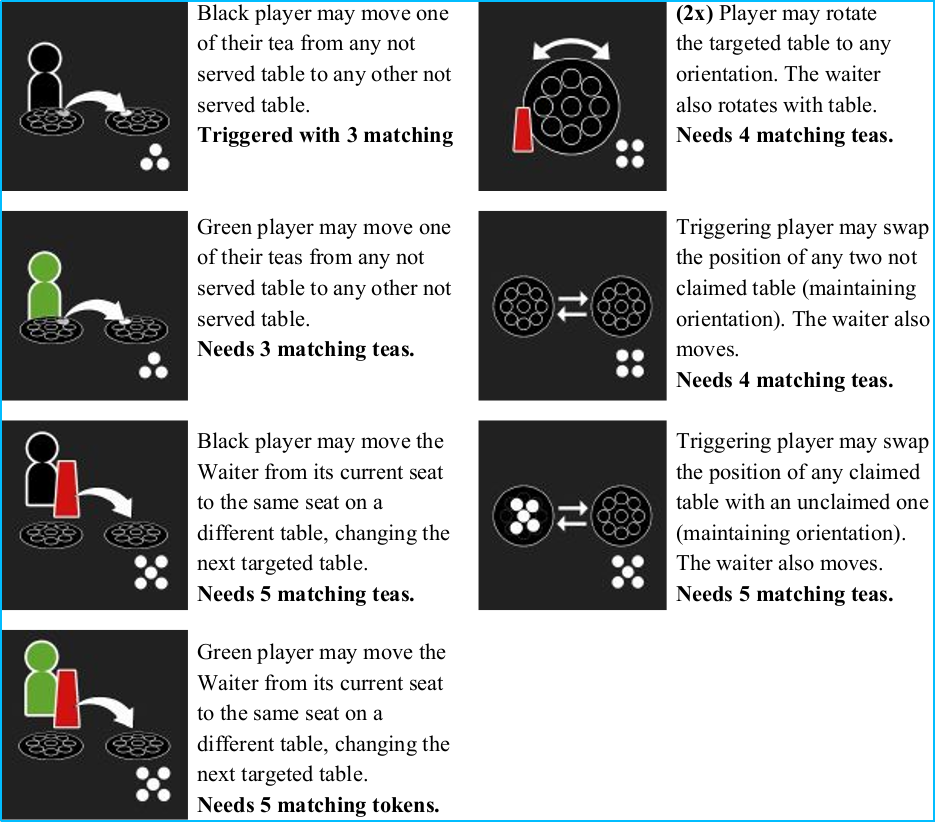
\includegraphics[width=\linewidth]{specials.png}
  \caption{Specials list.}\label{fig:specials}
\endminipage\hfill

\end{figure}




%%%%%%%%%%%%%%%%%%%%%%%%%%






\section{Game Logic}

Descrever o projeto e implementação da lógica do jogo em Prolog, incluindo a forma de representação do estado do tabuleiro e sua visualização, execução de movimentos, verificação do cumprimento das regras do jogo, determinação do final do jogo e cálculo das jogadas a realizar pelo computador utilizando diversos níveis de jogo. Sugere-se a estruturação desta secção da seguinte forma:

\subsection{Game State Representation} Pode ser idêntico ao descrito no relatório intercalar.)

\subsection{Board Visualization} (Pode ser idêntico ao descrito no relatório intercalar.)

\subsection{Lista de Jogadas Válidas} Obtenção de uma lista de jogadas possíveis. Exemplo: \textit{valid\_moves(+Board, -ListOfMoves)}.

\subsection{Turns} Validação e execução de uma jogada num tabuleiro, obtendo o novo estado do jogo. Exemplo: \textit{move(+Move, +Board, -NewBoard)}.

\subsection{Board Evaluation} Avaliação do estado do jogo, que permitirá comparar a aplicação das diversas jogadas disponíveis. Exemplo: \textit{value(+Board, +Player, -Value)}.

\subsection{End Game Verification} Verificação do fim do jogo, com identificação do vencedor. Exemplo: \textit{game\_over(+Board, -Winner)}.

\subsection{CPU Play}
    Nos jogos em que se escolhe a opção que contém AI, a escolha da jogada do computador  Por exemplo: \textit{choose\_move(+Level, +Board, -Move)}.


%%%%%%%%%%%%%%%%%%%%%%%%%%
\section{User Interface}

The code responsible for interfacing with the user is located in the module/file 'io.pl'.
It's a combination of 3 menus and the game interface.

\begin{figure}[!h]
\centering
\minipage[t]{0.23\textwidth}
  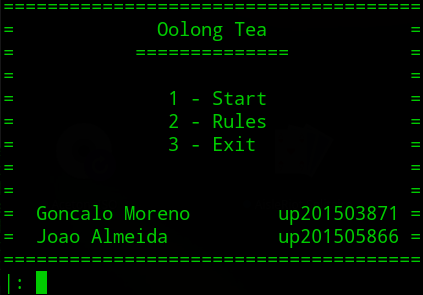
\includegraphics[width=\linewidth]{menu_inicial.png}
  \caption{Inicial Menu.}\label{fig:menu_inicial}
\endminipage
\minipage[t]{0.23\textwidth}
  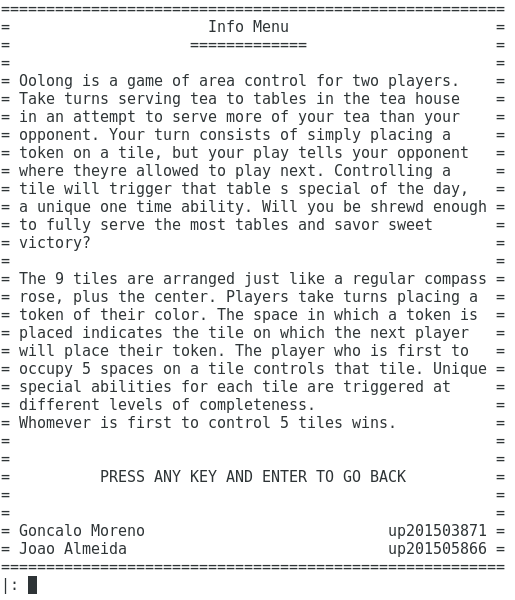
\includegraphics[width=\linewidth]{menu_info.png}
  \caption{Rules Menu.}\label{fig:menu_info}
\endminipage
\minipage[t]{0.23\textwidth}%
  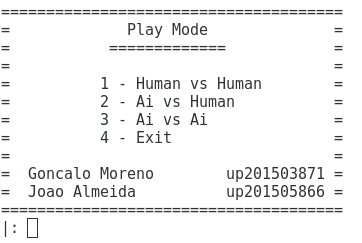
\includegraphics[width=\linewidth]{menu_play.png}
  \caption{Game Options.}\label{fig:menu_play}
\endminipage\hfill

\minipage{0.5\textwidth}%
    \vspace{0.7cm}
  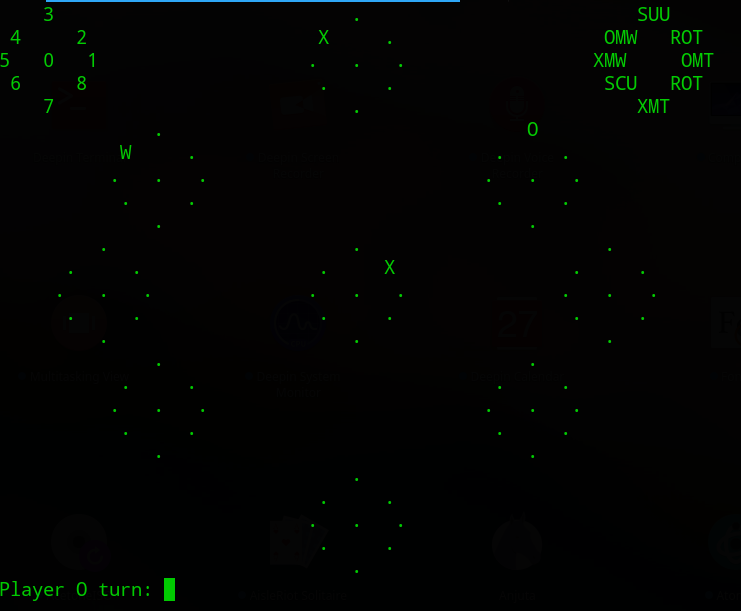
\includegraphics[width=\linewidth]{game.png}
  \caption{Game Interface.}\label{fig:game}
\endminipage\hfill

\end{figure}

The game interface is generated from a predicative that operates over the game board, represented by a list of lists.

\lstset{emph={%
   {:-}%
     },emphstyle={\color{red}\bfseries\underbar}%
}%

\renewcommand\listingscaption{Code}

\begin{listing}[!h]
    \caption{Interface Source Code}
    \label{Codigo:cod}
    \begin{minted}{prolog}

drawBoard(Board) :-
    Example = [0,1,2,3,4,5,6,7,8],
    at(L1,3,Board),
    at(Specials, 9, Board),
    space(4), drawST(Example), space(27), drawST(L1), space(25),
                                        drawSpecT(Specials), nl,
    space(1), drawSTM(Example), space(21), drawSTM(L1), space(19),
                                        drawSpecTM(Specials), nl,
    drawSM(Example), space(19), drawSM(L1), space(17),
                                        drawSpecM(Specials), nl,
    space(1), drawSBM(Example), space(21), drawSBM(L1), space(19),
                                        drawSpecBM(Specials), nl,
    space(4), drawSB(Example), space(27), drawSB(L1), space(25),
     drawSpecB(Specials), nl,

    at(L2,4,Board), at(L3,2,Board),
    space(14), drawST(L2), space(33), drawST(L3), nl,
    space(11), drawSTM(L2), space(27), drawSTM(L3), nl,
    space(10), drawSM(L2), space(25), drawSM(L3), nl,
    space(11), drawSBM(L2), space(27), drawSBM(L3), nl,
    space(14), drawSB(L2), space(33), drawSB(L3), nl,

    at(L4,5,Board), at(L5,0,Board), at(L6,1,Board),
    space(9), drawST(L4), space(22), drawST(L5), space(22),
                                                drawST(L6), nl,
    space(6), drawSTM(L4), space(16), drawSTM(L5), space(16),
                                                drawSTM(L6), nl,
    space(5), drawSM(L4), space(14), drawSM(L5), space(14),
                                                drawSM(L6), nl,
    space(6), drawSBM(L4), space(16), drawSBM(L5), space(16),
                                                drawSBM(L6), nl,
    space(9), drawSB(L4), space(22), drawSB(L5), space(22),
                                                drawSB(L6), nl,

    at(L7,6,Board), at(L8,8,Board),
    space(14), drawST(L7), space(33), drawST(L8), nl,
    space(11), drawSTM(L7), space(27), drawSTM(L8), nl,
    space(10), drawSM(L7), space(25), drawSM(L8), nl,
    space(11), drawSBM(L7), space(27), drawSBM(L8), nl,
    space(14), drawSB(L7), space(33), drawSB(L8), nl,

    at(L9,7,Board),
    space(32), drawST(L9), nl,
    space(29), drawSTM(L9), nl,
    space(28), drawSM(L9), nl,
    space(29), drawSBM(L9), nl,
    space(32), drawSB(L9), nl.

\end{minted}

\end{listing}



%%%%%%%%%%%%%%%%%%%%%%%%%%
\section{Conclusion}
Que conclui deste projecto? Como poderia melhorar o trabalho desenvolvido?




\clearpage
\addcontentsline{toc}{section}{Bibliografia}
\renewcommand\refname{Bibliografia}
\bibliographystyle{plain}
\bibliography{myrefs}

\newpage
\appendix
\section{Game Code}
Código Prolog implementado devidamente comentado e outros elementos úteis que não sejam essenciais ao relatório.

\end{document}
